% Nanyang Technological University - Qualification Examination report template
% 1st Draft 27/June/2014 (v.1.0) (Written by Ali Qasim - eng.amq@gmail.com)
% A modified version of Harvard thesis template
% ---------------------------------------------------------------------------- %
% Update v.1.1 26/August/2014 (Written by Ali Qasim - eng.amq@gmail.com)
% 1- Abstract moved to the beginning of the frontmatter.
% 2- Page numbering format for frontmatter changed to capitalized roman "Roman".
% 3- Cover page is a closer match to that provided by the faculty, with an empty page added after it.
% 4- Modified IEEE citation style to disable replacing author names with dashes in consecutive references with similar author names.

% ---------------------------------------------------------------------------- %
% Set Document Class
% ---------------------------------------------------------------------------- %
\documentclass[11pt,oneside,final]{ntu_qe}

\newcommand{\numcol}{1}
% ---------------------------------------------------------------------------- %
% Includes Packages
% ---------------------------------------------------------------------------- %
\usepackage{NTUdis}
\usepackage{setspace}
\usepackage{graphicx} 
\graphicspath{{Figures/}}
\usepackage{float}
\usepackage{subfigure}
\usepackage{algorithm}
\usepackage{amsfonts}
\usepackage{ifthen}
\usepackage{booktabs}
\usepackage{amssymb}
\usepackage{supertabular}
\usepackage{array}
\usepackage{multirow}
\usepackage{fancyhdr}
%\usepackage{fancyheadings}
\usepackage{psfrag}
\usepackage{amsmath}
\usepackage{hhline}
\usepackage{type1cm}
\usepackage{lettrine}
\usepackage{cite}
\usepackage{fancybox}
\usepackage{ctable}

% ---------------------------------------------------------------------------- %
% Math Equation Setting
% ---------------------------------------------------------------------------- %
\newtheorem{mydef}{Definition}
% ---------------------------------------------------------------------------- %
% Comment Setting
% ---------------------------------------------------------------------------- %
\usepackage[colorinlistoftodos]{todonotes}
% ---------------------------------------------------------------------------- %
% Document Setting
% ---------------------------------------------------------------------------- %
% Front Matters
% Labels : 1) All labels starts with fig, table, algo, eqn
% 2) use relative directory. current file name. name 
% fig:wdcdf.thesis.algo.tex.flow_chart
%

% define the following before \input this tex
% \newcommand{\numcol}{2}
\newcommand{\checkOneCol}{\ifthenelse{\numcol = 1}}

\newcommand{\tablefont}{\small}

% Wrapping functions 
\newcommand{\wchapter}{\chapter}
\newcommand{\wsection}{\section}
\newcommand{\wsubsection}{\subsection}
\newcommand{\wsubsubsection}{\subsubsection}

% -- abstract
\newcommand{\wabstract} {\begin{abstract}}
\newcommand{\wendabstract} {\end{abstract}}

% -- mathematics
\newcommand{\weqnarray}{\begin{eqnarray}}
\newcommand{\wendeqnarray} {\end{eqnarray}}
\newcommand{\waligneqnarray}{\begin{align}}
\newcommand{\walignendeqnarray} {\end{align}}

% -- lines
\newcommand{\emptyline}{\noindent\newline}
\newcommand{\emptyindentline}{\emptyline\indent}

% -- table
\newcommand{\wtable}{\begin{table}}
\newcommand{\wendtable}{\end{table}}

% -- figure
\newcommand{\wfigure}{\begin{figure}}
\newcommand{\wendfigure}{\end{figure}}

% -- list
\newcommand{\wlist}{\begin{itemize}}
\newcommand{\wendlist}{\end{itemize}}
\newcommand{\wdesc}{\begin{description}}
\newcommand{\wenddesc}{\end{description}}

% -- Number List
\newcommand{\wnumlist}{\begin{enumerate}}
\newcommand{\wendnumlist}{\end{enumerate}}

% String declaration for references
\newcommand{\lfig}{Fig.}
\newcommand{\ltable}{Table}
\newcommand{\lalgo}{Algorithm}
\newcommand{\leqn}{Eqn.}
\newcommand{\llemma}{Lemma}
\newcommand{\lcorollary}{Corollary}
\newcommand{\ltheorem}{Theorem}
\newcommand{\ldef}{Def.}
\newcommand{\lsection}{Section}
\newcommand{\lchapter}{Chapter}
\newcommand{\lappendix}{Appendix}
\newcommand{\lexample}{Example}
\newcommand{\lcase}{Case}
%
% Format for mathematics
\newtheorem{theorem}{Theorem}
\newtheorem{lemma}{Lemma}
\newtheorem{corollary}{Corollary}
\newtheorem{definition}{Definition}
\newtheorem{example} {Example}
\newtheorem{case} {Case}
%
\newcommand{\wtheorem}{\begin{theorem}}
\newcommand{\wendtheorem}{\end{theorem}}
\newcommand{\wlemma}{\begin{lemma}}
\newcommand{\wendlemma}{\end{lemma}}
\newcommand{\wcorollary}{\begin{corollary}}
\newcommand{\wendcorollary}{\end{corollary}}
\newcommand{\wdefinition}{\begin{definition}}
\newcommand{\wenddefinition}{\end{definition}}
\newcommand{\wexample}{\begin{example}}
\newcommand{\wendexample}{\end{example}}
\newcommand{\wproof}{\begin{proof}}
\newcommand{\wendproof}{\end{proof}}
\newcommand{\wcase}{\begin{case}}
\newcommand{\wendcase}{\end{case}}
%\renewcommand{\QED}{\QEDopen}
%

% - Spacing mode
\newcommand{\setsinglespace}{\ssp}
\newcommand{\setonehalfspace}{\hsp}
\newcommand{\setdoublespace}{\dsp}
% - Define the function "NewPage" to force create a new page when needed
\newcommand*\NewPage{\newpage\null\thispagestyle{empty}\newpage}
% ---------------------------------------------------------------------------- %
% Table Of Contents Setup
% - max depth listed:
% 1 = section, 2 = subsection, 3 = subsubsection
% ---------------------------------------------------------------------------- %
\setcounter{tocdepth}{3}

\begin{document}
\setdoublespace
% ---------------------------------------------------------------------------- %
% Title page
% includes -  Front and Second covers
% ---------------------------------------------------------------------------- %
%\pagestyle{empty}

% ----------------------------------------------------------------------------
% Title Page
% ----------------------------------------------------------------------------

\title{Project Title}
\author{Your Holy Name}
\degreemonth{Month} % month final submission occurs.
\degreeyear{Year}
\field{Electrical Engineering}
\department{School of Electrical and Electronics Engineering}
\school{Nanyang Technological University}
\advisor{Associate Professor Dr. Ali Nagaratnam Zhang}
\degreetype{M.Eng /  Ph.D}
\matricno{Matric Number}
\maketitle
%\copyrightpage
\hsp
\NewPage
% ---------------------------------------------------------------------------- %
% Front Matters
% includes - Table of Contents, Abstract, Acknowledgement, 
% List of Figures and List of Tables
% ---------------------------------------------------------------------------- %
% ---------------------------------------------------------------------------- %
% Front Matters
% ---------------------------------------------------------------------------- %
% ---------------------------------------------------------------------------- %
% Acknowledgement
% ---------------------------------------------------------------------------- %
% ---------------------------------------------------------------------------- %
% Abstract
% ---------------------------------------------------------------------------- %

\setsinglespace
\begin{nabstract}
%abstract
Ultra-wide band (UWB) indoor positioning always suffers from extremely high-rate signal detection. The compressive sensing (CS), which is considered as the optimal solution of acquisition and reconstruction for sparse signals, provides an alternative solution by implementing random projection at transmitters or receivers. However, these CS based UWB positioning systems still cannot avoid high-rate mixing operation when generating the PN sequence during random projection. In this paper, we propose a new CS based UWB positioning system to solve this problem, which implements a relatively low-rate random pre-mixing at the transmitter and correspondingly sub-Nyquist rate sampling at receivers. As a result, the new system successfully eliminates the extremely high Nyquist rate in the system by sacrifices a small degree of compression ratio. Simulation results demonstrate the new system maintains outstanding performance in terms of positioning accuracy. 

\newpage
\end{nabstract}

\setonehalfspace
\addcontentsline{toc}{section}{Table of Contents}
\tableofcontents
\listoffigures
\listoftables

\newpage
\startarabicpagination
%END

%\setdoublespace
% ---------------------------------------------------------------------------- %
\hsp
\chapter{Introduction}\label{CH1} %Chapter 1 - Introduction
\section{Background}

Background text...

\subsection{SubSection}

bla bla bla..

\subsubsection{SubSubSection}

\section{Motivation and Objectives}

Motivations.. and.. objectives..

\subsection{SubSection}

Bla bla..

\subsubsection{SubSubSection}

Bla bla..

\subsection{Objectives}

The objectives are.. ta ra ra raaa

\section{Organization of the Report}

The report is organized as follows:

\begin{enumerate}
\item Chapter \ref{CH1} introduces bla bla
\item Chapter \ref{CH2} shows bla bla
\item Chapter \ref{CH3} shows bla bla
\item Chapter \ref{CH4} demonstrates bla bla
\item Chapter \ref{CH5} draws a conclusion for the report and introduces ideas for future work.
\end{enumerate}
% ---------------------------------------------------------------------------- %
% Chapter 2 - 
\chapter{Literature Review}\label{CH2}
\section{Introduction}

Introduction..

\section{First Section}

According to \cite{BibtexKey}, bla bla..

\begin{figure}[tbh]
\begin{center}
\noindent
  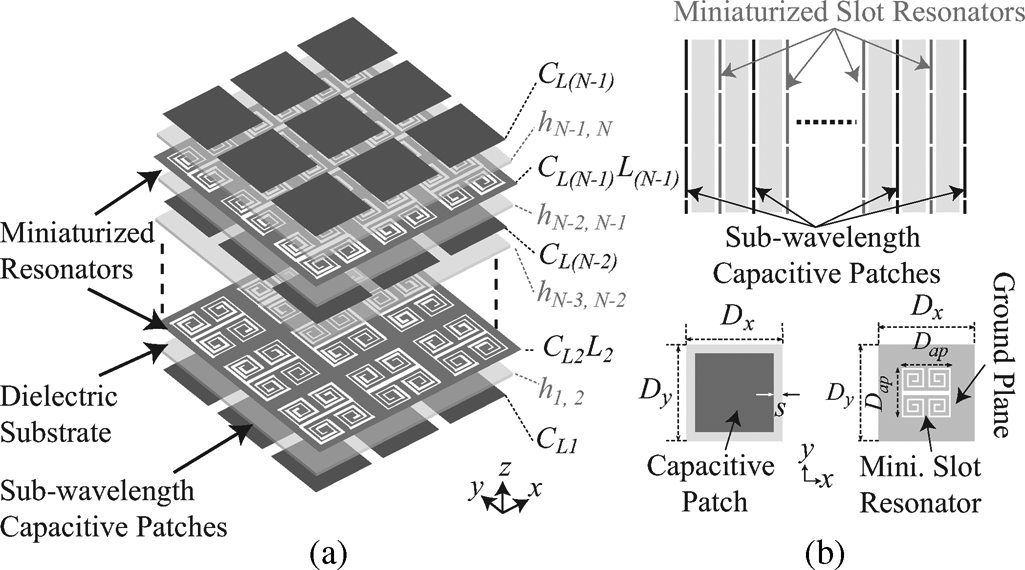
\includegraphics[width=0.7\textwidth]{FigureA}
  \end{center}
    \caption{FigureA's caption.}\label{FigureA}
\end{figure}

\section{Second Section}

Bla bla..

\begin{figure}[tbh]
\begin{center}
\noindent
  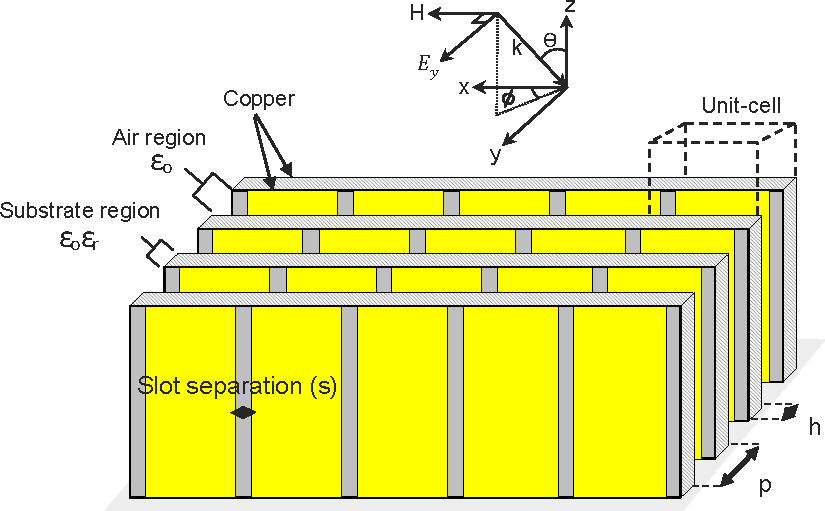
\includegraphics[width=0.7\textwidth]{FigureB}
  \end{center}
    \caption{FigureB's caption.}\label{FigureB}
\end{figure}

\section{Conclusion}

In conclusion, everything has been bla bla all over.

% ---------------------------------------------------------------------------- %
% Chapter 3 - 
\chapter{First Proposed Solution}\label{CH3}
\section{Introduction}

Introduction..

\section{Our Proposed Solution}\label{Ch3:ProposedSol}

Our proposed solution is..

\subsection{Design and Analysis}\label{Ch3:Analysis}

The design process starts by..

\subsection{Design Example} \label{Ch3:Example}

The design example we proposed is.. 

\subsubsection{Theory and Procedures}\label{Ch3:Theory}

The theory states that..

\subsubsection{Simulated and Measured Results}\label{Ch3:Measured}

The results shown in..

\section{Our Second Proposed Solution}

Bla bla..

\subsection{Design and Analysis}

Bla bla..

\subsection{Design Example}

Bla bla..

\subsubsection{Theory and Procedures}

Bla bla..

\subsubsection{Simulated and Measured Results}

Bla bla..

\section{Conclusion}

In conclusion, and as before, most of it has been bla bla..
% ---------------------------------------------------------------------------- %
% Chapter 4 - 
\chapter{Second Proposed Solution}\label{CH4}
\section{Introduction}

Introduction..

\section{Description of the Solution}

Bla bla..

\section{Design Example}

Bla bla..

\subsection{Theory and Procedures}

Bla bla..

\subsection{Simulated and Measured Results}

Bla bla..

\section{Conclusion}

And the conclusion is, same old same!
% ---------------------------------------------------------------------------- %
% Chapter 5 - 
\chapter{Conclusion and Future Work}\label{CH5}
\section{Introduction}

Introduction..

\section{Description of the Solution}

Bla bla..

\section{Design Example}

Bla bla..

\subsection{Theory and Procedures}

Bla bla..

\subsection{Simulated and Measured Results}

Bla bla..

\section{Conclusion}

And the conclusion is, same old same!
%
---------------------------------------------------------------------------- %
% Chapter 6 - 
\chapter{Conclusion and Future Work}\label{CH6}
\section{Conclusion}

In conclusion, as Brad Pitt and his chio wife said in \cite{BibtexKey}, NTU researchers have no life. So, go get a life!

\section{Future Work}

A few suggestions are provided for related future works:

\begin{enumerate}

\item Bla.. 

\item Bla..

\item Bla..

\end{enumerate}
% ---------------------------------------------------------------------------- 
%
% List of Publications
%\addcontentsline{toc}{chapter}{List of Publications}
\renewcommand{\bibname}{List of Publications}
\begin{thebibliography}{1}

\bibitem{} NTUnerd and NTUBigNerd, "An Approach to Reserve Tickets to Phuket While Your Supervisor is On Leave," \emph{Whateverth Singaporean Conf. on Nerdy Yet Sexy Researchers (SgNYSR), 20whateverteen, pp. xxxx-xxxx}.

\end{thebibliography}
% ---------------------------------------------------------------------------- %
% Bibliography
% ---------------------------------------------------------------------------- %
\ssp
\renewcommand{\bibname}{References}
\bibliography{APPENDIX/References}
% ---------------------------------------------------------------------------- %
% Appendix 
\newpage
\appendix
% ---------------------------------------------------------------------------- % 
% Appendix A - 
% ---------------------------------------------------------------------------- %
\section{The Null Space Property}\label{Ch2:NSP}

Our proposed solution is..

% ---------------------------------------------------------------------------- %
% Appendix B - 
% ---------------------------------------------------------------------------- %
%\input{..}
% ---------------------------------------------------------------------------- %
\end{document}
% ---------------------------------------------------------------------------- %